\chapter{Wykorzystane algorytmy i ich charakterystyka}
\textit{Autor: Bartosz Kołakowski}
\setlength{\parindent}{0pt}

\section{Szyfrowanie symetryczne}
\subsection{Opis szyfrowania symetrycznego}
Szyfrowanie symetryczne (inaczej szyfrowani z kluczem tajnym czy szyfrowanie z kluczem pojedynczym) jest rodzajem szyfrowania, gdzie do operacji szyfrowania jak i deszyfrowania wykorzystywany jest tylko jeden klucz. W przeciwieństwie do klucza publicznego w szyfrowaniu asymetrycznym klucz w szyfrowaniu symetrycznym jest tajny i nie powinien być nikomu ujawniany. Istnieje wiele algorytmów szyfrowania symetrycznego, są to na przykład Twofish, Serpent czy AES. W tej implementacji został wybrany AES, który jest jednym z najczęściej używanych algorytmów klucza pojedynczego. Jego zaletami jest bezpieczeństwo i odporności na złamanie szyfru, o których zostanie napisane w dalszej części pracy. Inną cechą tego algorytmu jest jego wydajność, w porównaniu do innych algorytmów szyfrowania symetrycznego (w porównaniu do algorytmów szyfrowania asymetrycznego oczywiście też, ale kryptografia klucza publicznego jest kilka rzędów wolniejsza od kryptografii z jednym kluczem). Między innymi to wydajność AES (bezpieczeństwo oczywiście też) była cechą, która sprawiła, że został on wybrany nad algorytmami Serpent, Twofish, RC6 i MARS. Algorytmy te same w sobie również były bezpieczne, ale ich gorsza wydajność sprawiła, że to nie one zostały w 2001 wybrane przez National Institute of Standards and Technology na następcę DES. Inną ważną cechą AES jest jego powszechne stosowanie i popularność, jest on między innymi wykorzystywany w protokołach TLS (Transport Layer Security), IPsec (Internet Protocol Security) czy WPA (WiFi Protected Access).

Szyfrowanie symetryczne pokazane jest na rysunku \ref{fig:AES1}
\begin{figure}[H]
    \centering
    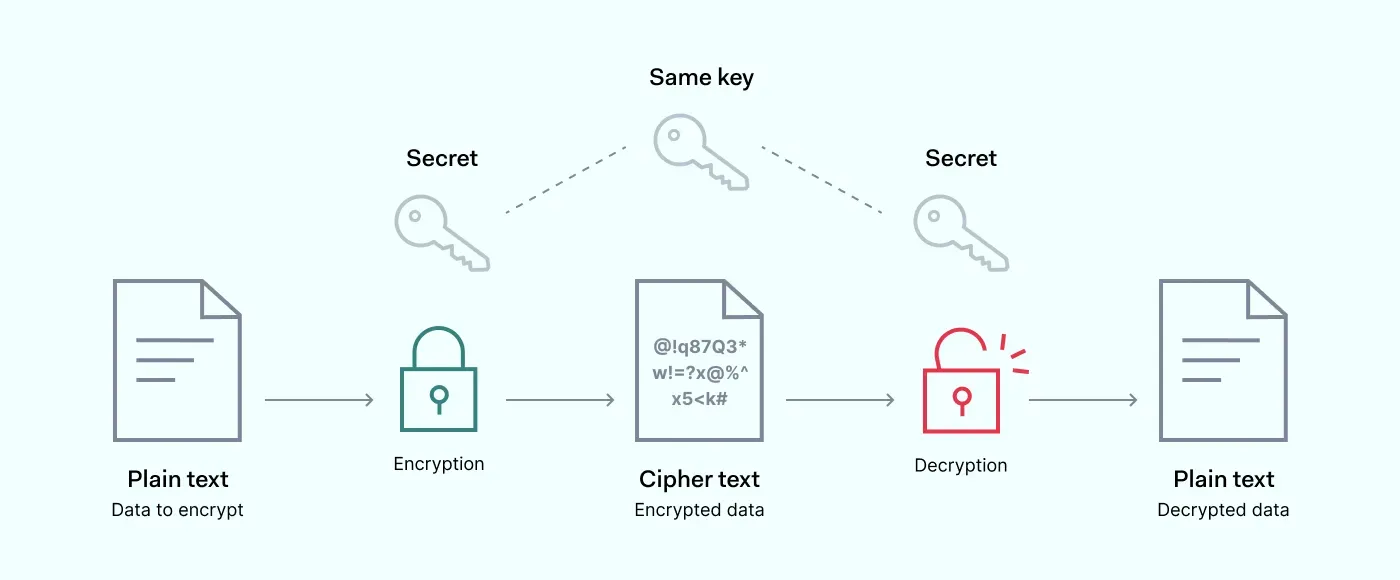
\includegraphics[width=\textwidth]{Images/AES1.png}
    \caption{Schemat szyfrowania symetrycznego}
    \label{fig:AES1}
\end{figure}

Algorytm AES (skrót od Advanced Encryption Standard) jest jednym z najbardziej znanych algorytmów kryptografii symetrycznej. Jego zdecydowaną zaletą jest fakt, że ten algorytm jest dobrze przetestowany i powszechnie używany. Jego historia opiera się na tym, że wcześniej powszechnie używany algorytm DES (Data Encryption Standard) nie zapewniał już odpowiedniego poziomu bezpieczeństwa, między innymi przez krótką długość klucza i małą długość bloku co powodowało niską odporność na ataki. W konkursie ogłoszonym przez NIST (skrót od National Institute of Standards and Technology) mającym zastąpić DES wygrał algorytm, którego oryginalna nazwa brzmiała Rijndael. Aby zrozumieć, dlaczego AES został wybrany i jest tak powszechnie stosowany zostanie przedstawione jak działa i zobaczyć jego charakterystyczne cechy.

\vspace{0.3\baselineskip}

Tak jak wcześniej wspomniano AES jest algorytmem szyfrowania symetrycznego, który opiera się na blokach. Mają one stały rozmiar 128 bitów. Cały algorytm opiera się na wielu matematycznych operacjach, które są podzielone na rundy. To, ile jest rund zależy od tego jaka jest długość (10 rund dla klucza 128-bitowego, 12 rund dla klucza 192-bitowego, 14 rund dla klucza 256-bitowego). Operacje są wykonywane na macierzach 4x4 bajty.

\vspace{0.3\baselineskip}

Operacje wykonywane w każdej z rund przedstawiają się następująco:
\begin{enumerate}
    \item Zamiana bajtów – zamiana każdego bajtu według schematu w tabeli podstawień, ma to na celu to, żeby te operacje były nieliniowe,
    \item Zamiana wierszy – przesunięcie określonej ilości wierszy macierzy, w celu dyfuzji danych
    \item Mieszanie kolumn – jest to osiągnę przez mnożenie elementów tych kolumn
    \item Dodanie klucza – do macierzy dodawany jest klucz rundowy (głównie przez wykorzystanie operacji alternatywy rozłącznej)
\end{enumerate}
Wszystkie te operacje mają na celu zaciemnienie oryginalnych danych tak, żeby nie dało się ich odszyfrować bez znajomości symetrycznego klucza, a fakt, że operacje są wykonywane w wielu rundach czyni algorytm jeszcze bardziej trudniejszym do złamania.

\vspace{0.3\baselineskip}

Jak wyglądają operacje w algorytmie AES pokazane jest na rysunku \ref{fig:AES2}
\begin{figure}[H]
    \centering
    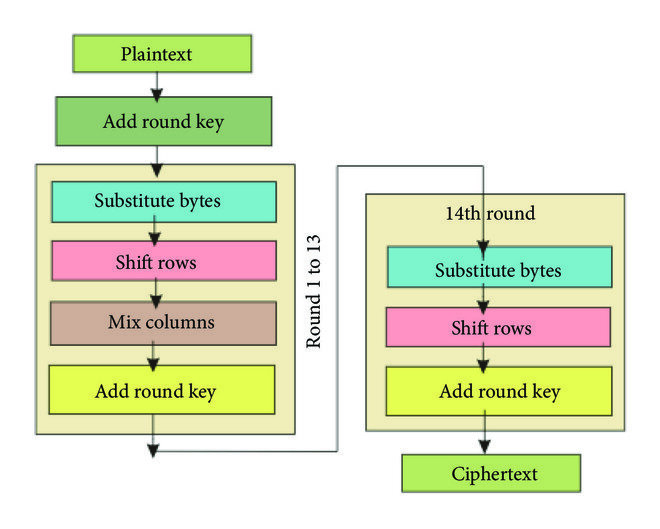
\includegraphics[width=\textwidth]{Images/AES2.jpg}
    \caption{Schemat działania AES}
    \label{fig:AES2}
\end{figure}

\subsection{Użycie szyfrowania symetrycznego w praktyce}

\begin{lstlisting}[caption={Szyfrowanie danych}]
def encrypt_data_ecb(data, key):
    cipher = AES.new(key, AES.MODE_ECB)
    encrypted_data = cipher.encrypt(pad(data.encode(), AES.block_size))
    encrypted_base64 = base64.b64encode(encrypted_data).decode('utf-8')
    return encrypted_base64
\end{lstlisting}
\listings{Szyfrowanie danych}
Szyfrowanie danych odbywa się przez funkcję, której parametrami są tekst podany do zaszyfrowania oraz klucz sesyjny. W samej funkcji najpierw tworzony jest obiekt szyfrujący AES, który jest ustawiony w trybie wiązania bloków zaszyfrowanych ECB - Electronic CodeBook (Tryb Elektronicznej Książki Kodowej). Dlaczego akurat w takim trybie, a nie na przykład CBC - Cipher Block Chaining (Tryb Wiązania Bloków Zaszyfrowanych), CFB - Cypher Feed Back (Tryb Sprzężenia Zwrotnego Szyfrogramu) czy OFB - Output Feedback (Tryb Sprzężenia Zwrotnego Wyjścia) - powodem jest charakterystyka tego trybu - pożądaną cechą w systemie jest to, aby był on deterministyczny, co wyklucza elementy losowe, a ECB jako jedyny z powszechnie używanych trybów wiązania bloków zaszyfrowanych nie korzysta z losowych wektorów inicjalizujących. Następnie szyfrujemy z wykorzystaniem wcześniej stworzonego obiektu szyfrującego, a wynik tej operacji przekonwertowujemy do łańcucha znaków za pomocą Base64.

\begin{lstlisting}[caption={Deszyfrowanie danych}]
def decrypt_data_ecb(encrypted_base64, key):
    encrypted_data = base64.b64decode(encrypted_base64)
    cipher = AES.new(key, AES.MODE_ECB)
    decrypted_data = unpad(cipher.decrypt(encrypted_data), AES.block_size)
    return decrypted_data.decode()
\end{lstlisting}
\listings{Deszyfrowanie danych}
W funkcji deszyfrującej najpierw zaszyfrowane dane są konwertowane z formatu Base64 na ciąg bajtów, potem podobnie jak w operacji szyfrowania tworzony jest nowy obiekt szyfrujący, którego tryb wiązania bloków zaszyfrowanych to ECB. Następnie deszyfrujemy dane za pomocą klucza sesyjnego i usuwamy zbędne wypełnienie.

\section{Szyfrowanie asymetryczne}

\subsection{Opis szyfrowania asymetycznego}
Szyfrowanie asymetryczne (inaczej nazywane szyfrowaniem klucza publicznego) to rodzaj szyfrowania, w którym występują dwa klucze – prywatny i publiczny. Klucz prywatny jest generowany na podstawie odpowiednio dużych liczb pierwszych i nie powinien być nikomu udostępniany. W kryptografii asymetrycznej klucz prywatny służy do odszyfrowywania. Drugim kluczem jest klucz publiczny, który jest generowany na podstawie klucza prywatnego i może on być udostępniany innym użytkownikom. Klucz publiczny w kryptografii klucza tajnego wykorzystywany jest przy szyfrowaniu. Jest wiele algorytmów kryptografii asymetrycznej – RSA, ElGamal czy Elliptic Curve Cryptography. W tej implementacji wykorzystano jeden z najczęściej wykorzystywanych algorytmów – jest to RSA. Algorytm RSA (jest to skrót od Rivest–Shamir–Adleman) jest jednym z najbardziej popularnych i najczęściej wykorzystywanych algorytmów kryptografii asymetrycznej. Jego istotnymi zaletami są bezpieczeństwo i wysoka odporność na ataki.

Zobrazowanie szyfrowania symetrycznego na grafice \ref{fig:RSA1}
\begin{figure}[H]
    \centering
    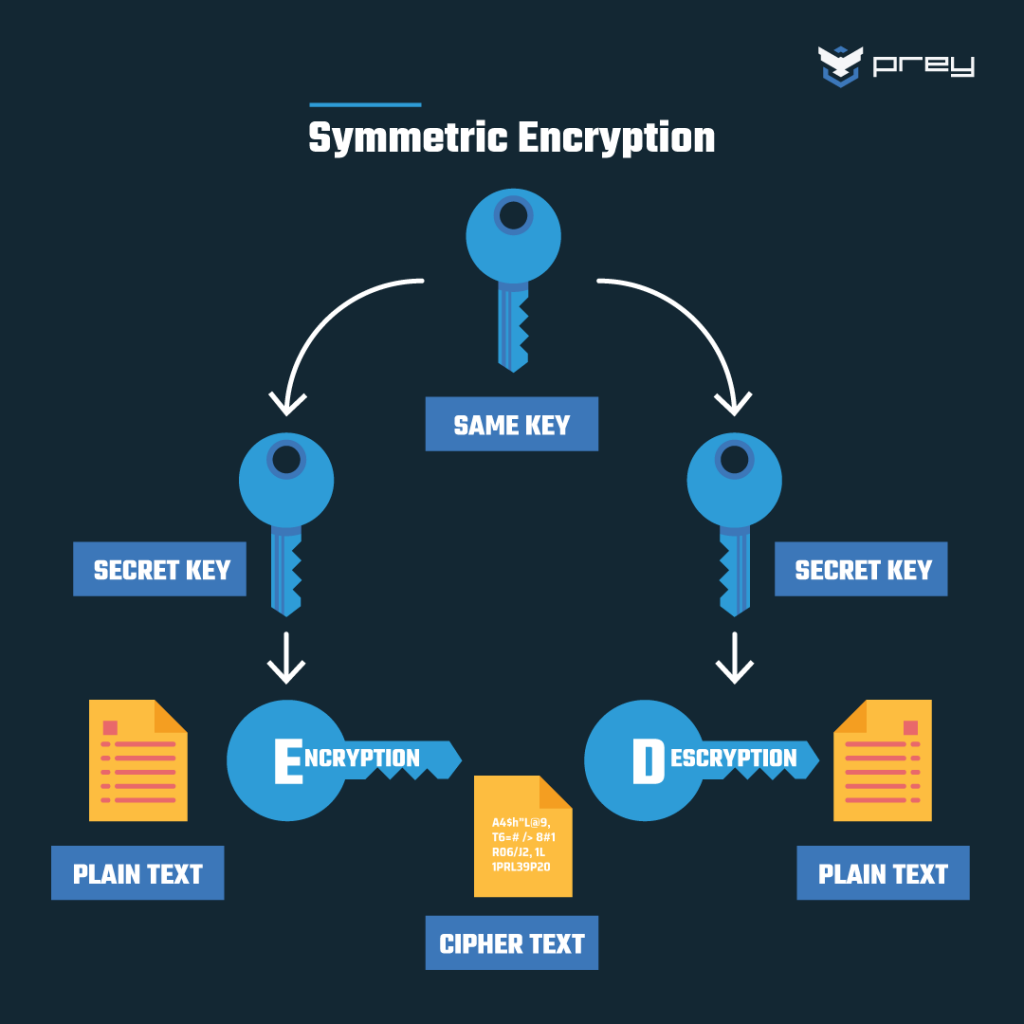
\includegraphics[width=\textwidth]{Images/RSA1.png}
    \caption{Schemat szyfrowania symetrycznego}
    \label{fig:RSA1}
\end{figure}

\vspace{0.3\baselineskip}

Szczegółowe działanie algorytmu RSA polega na tym, że wybiera się dwie duże liczby pierwsze, z których potem oblicza się moduł n i wartość z funkcji Eulera na podstawie tego modułu. Klucz publiczny jest liczbą względnie pierwszą do wartości funkcji Eulera. Klucz prywatny jest odwrotnością multiplikatywną wartości klucza publicznego modulo wartości funkcji Eulera. Szczegółowo przedstawia się to na wzorach:

Oznaczenie początkowych liczb - wzór \ref{eq:first}
\begin{equation}
    p, \; q-losowe, \; ogromne \; liczby \; pierwsze
    \label{eq:first}
\end{equation}
\equations{Oznaczenie początkowych liczb}
Wartość modułu - wzór \ref{eq:second}
\begin{equation}
    n=p*q
    \label{eq:second}
\end{equation}
\equations{Wartość modułu}
Wartość funkcji Eulera - wzór \ref{eq:third}
\begin{equation}
    \phi(n)=(p-1)*(q-1)
    \label{eq:third}
\end{equation}
\equations{Wartość funkcji Eulera}
Klucz publiczny - wzór \ref{eq:fourth}
\begin{equation}
    e \in \{NWD(\phi(n),e)=1, \; 1 \leqslant e \leqslant \phi(n)\}
    \label{eq:fourth}
\end{equation}
\equations{Klucz publiczny}
Klucz prywatny - wzór \ref{eq:fifth}
\begin{equation}
    d= e^{-1} (mod \; \phi(n))
    \label{eq:fifth}
\end{equation}
\equations{Klucz prywatny}
Szyfrowanie wiadomości odbywa się korzystając ze wzoru \ref{eq:sixth}
\begin{equation}
    C= M^e, \; C-zaszyfrowana \;  wiadomość, \; M-oryginalny \; tekst, \; e-klucz \; publiczny
    \label{eq:sixth}
\end{equation}
\equations{Szyfrowanie wiadomości}
Deszyfrowanie odbywa się za pomocą wzoru \ref{eq:seventh}
\begin{equation}
    M= C^d, \; M-deszyfrowana \; wiadmość, \;C-zakodowany \; tekst, \; d-klucz \; prywatny
    \label{eq:seventh}
\end{equation}
\equations{Deszyfrowanie wiadomości}
Bezpieczeństwo tego algorytmu opiera się na tym, że odwrócenie tych operacji i uzyskanie klucza prywatnego na podstawie czyjegoś klucza publicznego oraz treści zaszyfrowany i deszyfrowanych wiadomości jest obliczeniowo bardzo trudne.

Ukazanie RSA w skomplikowanych systemach na rysunku \ref{fig:RSASieci}
\begin{figure}[H]
    \centering
    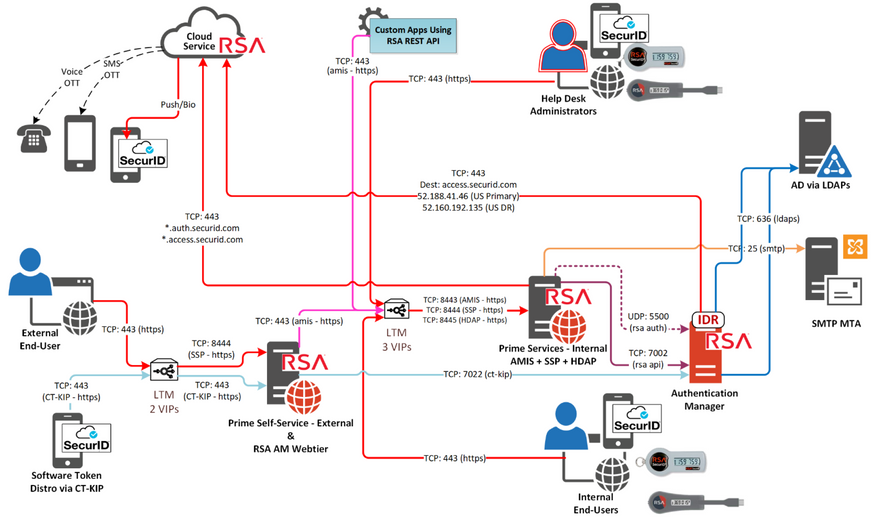
\includegraphics[width=\textwidth]{Images/RSASieci.png}
    \caption{Pokazanie RSA w zaawansowanych systemach}
    \label{fig:RSASieci}
\end{figure}

\subsection{Użycie szyfrowania asymetrycznego w praktyce}
\begin{lstlisting}[caption={Generowanie klucza prywatnego}]
self.private_key = rsa.generate_private_key(
            public_exponent=65537,
            key_size=2048,
            backend=default_backend()
)
\end{lstlisting}
\listings{Generowanie klucza prywatnego}

Każdy z użytkowników posiada wygenerowany klucz prywatny, jest on generowany losowo i niezależnie od innych. Inni użytkownicy nie wiedzą jaki jest klucz prywatny danego użytkownika. W stosowanej przez implementacji wykładnik publiczny ma zalecaną wartość dosyć małej liczby pierwszej (65537), a długość klucza to 2024 bitów, co sprawia, że algorytm jest wydajniejszy (to pokazuje różnicę między kryptografią asymetryczną, a kryptografią jednego klucza, gdzie jego długość w standardowych formatach AES to co najwyżej 256 bitów).


\begin{lstlisting}[caption={Generowanie klucza publicznego}]
self.public_key = self.private_key.public_key()
\end{lstlisting}
\listings{Generowanie klucza publicznego}

Klucz publiczny jest generowany na podstawie klucza publicznego, gdyż w kryptografii asymetrycznej klucze są między sobą powiązane.
\begin{figure}[H]
    \centering
    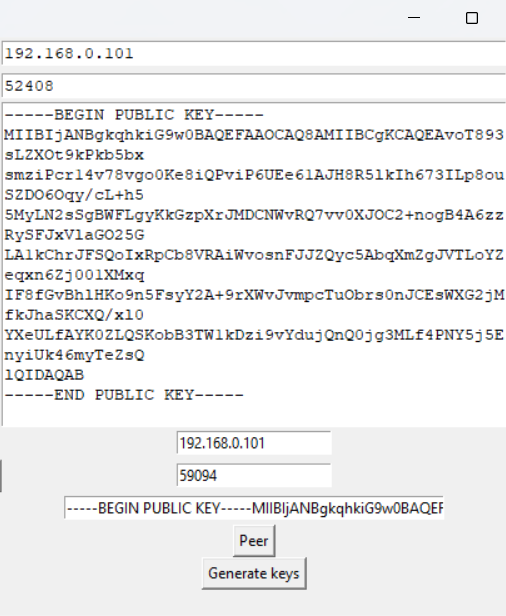
\includegraphics[width=\textwidth]{Images/CodeX13.png}
\end{figure}
Aby skutecznie połączyć się i komunikować się z innym użytkownikiem potrzebna jest znajomość jego klucza publicznego, dlatego w implementacji systemu przy nawiązywaniu połączenia podawany jest klucz publiczny (z którym nie ma żadnego zagrożenia bezpieczeństwa, aby został upubliczniony dla innych, w przeciwieństwie do klucza prywatnego).

\vspace{0.3\baselineskip}

W implementacji systemu pojawił się następującym problemem, mianowicie pożądane jest, aby wiadomości wysyłane przez sieć były łatwo dostępne dla innych użytkowników, którzy są członkami sieci, ale żeby ich treść nie była dostępna dla osób z zewnątrz (nie można ich przesyłać przez sieć jako zwykły tekst, ponieważ wtedy istniałaby możliwość podsłuchania i zostałby zaburzony jeden z filarów naszego systemu, czyli poufność wiadomości). Z tego powodu szyfrowanie wiadomości odbywa się w sposób symetryczny. Jednakże teraz może pojawić się pytanie czym będzie klucz w szyfrowaniu z pojedynczym kluczem i jak go ustalić w sposób bezpieczny. Tu jako rozwiązaniem jest szyfrowanie asymetryczne.

Każdy z użytkowników generuje losowy klucz sesyjny i w momencie powiększania się grupy (dodania nowego użytkownika) lub jej się zmniejszenia (usunięcie jednego z użytkowników) klucz sesyjny generuje się na nowo. Potem jeden z użytkowników jest w momencie zmiany składu grupy wybierany jako osoba mająca rozesłać klucz sesyjny.


\begin{lstlisting}[caption={Wybieranie osoby mającej rozesłać klucz sesyjny}]
def drawPerson(self):
    keyList = []
    for peer in self.peers:
        addrPort = {"addr": peer.addr, "port": peer.port}
        keyList.append(addrPort)
    myAddrPort = {"addr": ip(), "port": self.port}
    keyList.append(myAddrPort)
    sortedAddrPortList = sorted(keyList, key=lambda x: x["port"])
    keyRaw = " ".join(str(x["port"]) for x in keyList)
    self.drawString = keyRaw
    numeric_seed = int.from_bytes(hashlib.
    sha256(keyRaw.encode('utf-8')).digest())
    random.seed(numeric_seed)
    chosen_addr_port = random.choice(sortedAddrPortList)
    return chosen_addr_port
\end{lstlisting}
\listings{Wybieranie osoby mającej rozesłać klucz sesyjny}

Tak samo jak w przypadku Dowodu Stawki mechanizm losowania osoby mającej wysyłać klucz sesyjnym innym musi być taka sama dla wszystkich, tak oby osoba wysyłająca była w każdej instancji programu taka sama, inaczej użytkownicy mieliby różne klucze sesyjne co uniemożliwiłoby komunikację. Tworzy się lista użytkowników, którą następnie jest sortowana, aby każdy program miał ją w takiej samej postaci. Potem lista zamieniana jest na łańcuch znaków i używając deterministycznej funkcji skrótu (zwracającej te same wyniki dla tych samych danych) hashlib.sha256 (a nie na przykład domyślnej funkcji hash() w Pythonie, która nie jest deterministyczna) uzyskiwana jest wartość, która będzie ziarnem dla generatora liczb losowych i następnie wylosowany przez ten generator użytkownik (za pomocą standardowej funkcji random.choice()) będzie taki sam we wszystkich instancjach programu.

\begin{lstlisting}[caption={Uaklualnienie klucza sesyjnego}]
def update_group_session_key(self):
    self.EncryptedKBytes = encrypt_with_public_key
    (self.public_key, self.random_key)
    self.EncryptedKString = base64.b64encode(self.
    EncryptedKBytes).decode('utf-8')
    for peer in self.peers:
        peer.EncryptedKBytes = encrypt_with_public_key
        (peer.PKBytes, self.random_key)
        self.EncryptedKString = base64.b64encode
        (peer.EncryptedKBytes).decode('utf-8')
\end{lstlisting}
\listings{Uaklualnienie klucza sesyjnego}
Następnie po wylosowaniu osoby będącej odpowiedzialną za wysyłanie klucza ta osoba rozsyła do siebie klucz sesyjny zaszyfrowany swoim własnym kluczem publicznym, a do innych osób w sieci (biorąc pod uwagę niezmiennik, że każdy z każdym w danej grupie jest połączony) rozsyła klucz sesyjny zaszyfrowany kluczem publicznym danej osoby (właśnie dlatego, przy nawiązywaniu połączenia klucz podawany jest klucz publiczny – inaczej nie dało by się przekazać innym klucza sesyjnego z zachowaniem poufności). Dodatkową informacją godną uwagi jest fakt, że przy wysyłaniu innym zakodowanego klucza sesyjnego jest on poprzedzany nagłówkiem w celu łatwiejszego odebrania przez adresatów wiadomości.

\begin{lstlisting}[caption={Deszyfrowanie klucza sesyjnego}]
def convert_key(base64keyEncypted):
    byteKey = base64.b64decode(base64keyEncypted)
    decryptedSessionKey = me.private_key.decrypt(
        byteKey,
        padding.OAEP(
            mgf=padding.MGF1(algorithm=hashes.SHA256()),
            algorithm=hashes.SHA256(),
            label=None
        ))
    return decryptedSessionKey
\end{lstlisting}
\listings{Deszyfrowanie klucza sesyjnego}
Każdy z odbiorców po otrzymaniu klucza sesyjnego zakodowanego przez klucz publiczny w formacie Base64, korzysta z funkcji konwertującej,.pierwszą operacją jest zamienienie z typu łańcuchu znaków na format ciągu bajtów. Potem przebiega typowa dla kryptografii asymetrycznej operacja deszyfrowania kluczem prywatnym danego użytkownika, jednak szczególnie ważnym w niej jest fakt, że jest ona deterministyczna dla tych samych danych wejściowych do odszyfrowania, co oznacza, że jeśli podamy klucz sesyjny zaszyfrowany kluczem publicznym danego użytkownika i odszyfrujemy go jego kluczem prywatnym to zawsze wyjdzie nam poprawny klucz sesyjny z początku procesu. Ten klucz będzie potem wykorzystywany do odszyfrowania pojedynczych wiadomości w bloku przy wykorzystywaniu kryptografii klucza tajnego.

\section{Algorytmy osiągania konsensusu}
W kryptowalutach stosuje się wiele metod konsensusu z czego najbardziej popularne z nich to Dowód Pracy i Dowód Stawki, ale inne również znane to Dowód Pojemności i Delegowany Dowód Stawki. Aby uzasadnić która z nich została zastosowana w implementacji systemu, warto przeanalizować wszystkie z nich i zobaczyć ich wady i zalety.
\subsection{Dowód Pracy}
Dowód Pracy (angielski - Proof of Work) jest jedną z najstarszych metod konsensusu stosowanych w kryptowalutach gdzie dla każdego bloku wiadomości przypisana jest określona funkcja skrótu i użytkownicy mają za zadanie znaleźć odpowiednią funkcję skrótu, która spełnia określone wymagania (na przykład zaczyna się od konkretnej liczby zer). Z początku wydaje się, że ta metoda konsensusu ma dużo zalet, ponieważ każdy może wziąć udział w weryfikowaniu bloku, ale prawda jest taka, że przewagę w tym systemie mają osoby mające odpowiednio duże moce obliczeniowe, co prowadzi do centralizacji górnictwa przez firmy/organizacje posiadające ogromne ilości sprzętu oraz ogromnego zużycia energii i niekorzystnych zjawisk ekonomicznych takich jak gwałtowny wzrost cen kart graficznych (spowodowanych tym, że potrafią wykonywać dużo obliczeń w krótkim okresie czasu, co jest niezmiernie przydatne dla górników).

\vspace{0.3\baselineskip}

Działanie Dowodu Pracy na grafice \ref{fig:ConsesnsusProofOfWork}
\begin{figure}[H]
    \centering
    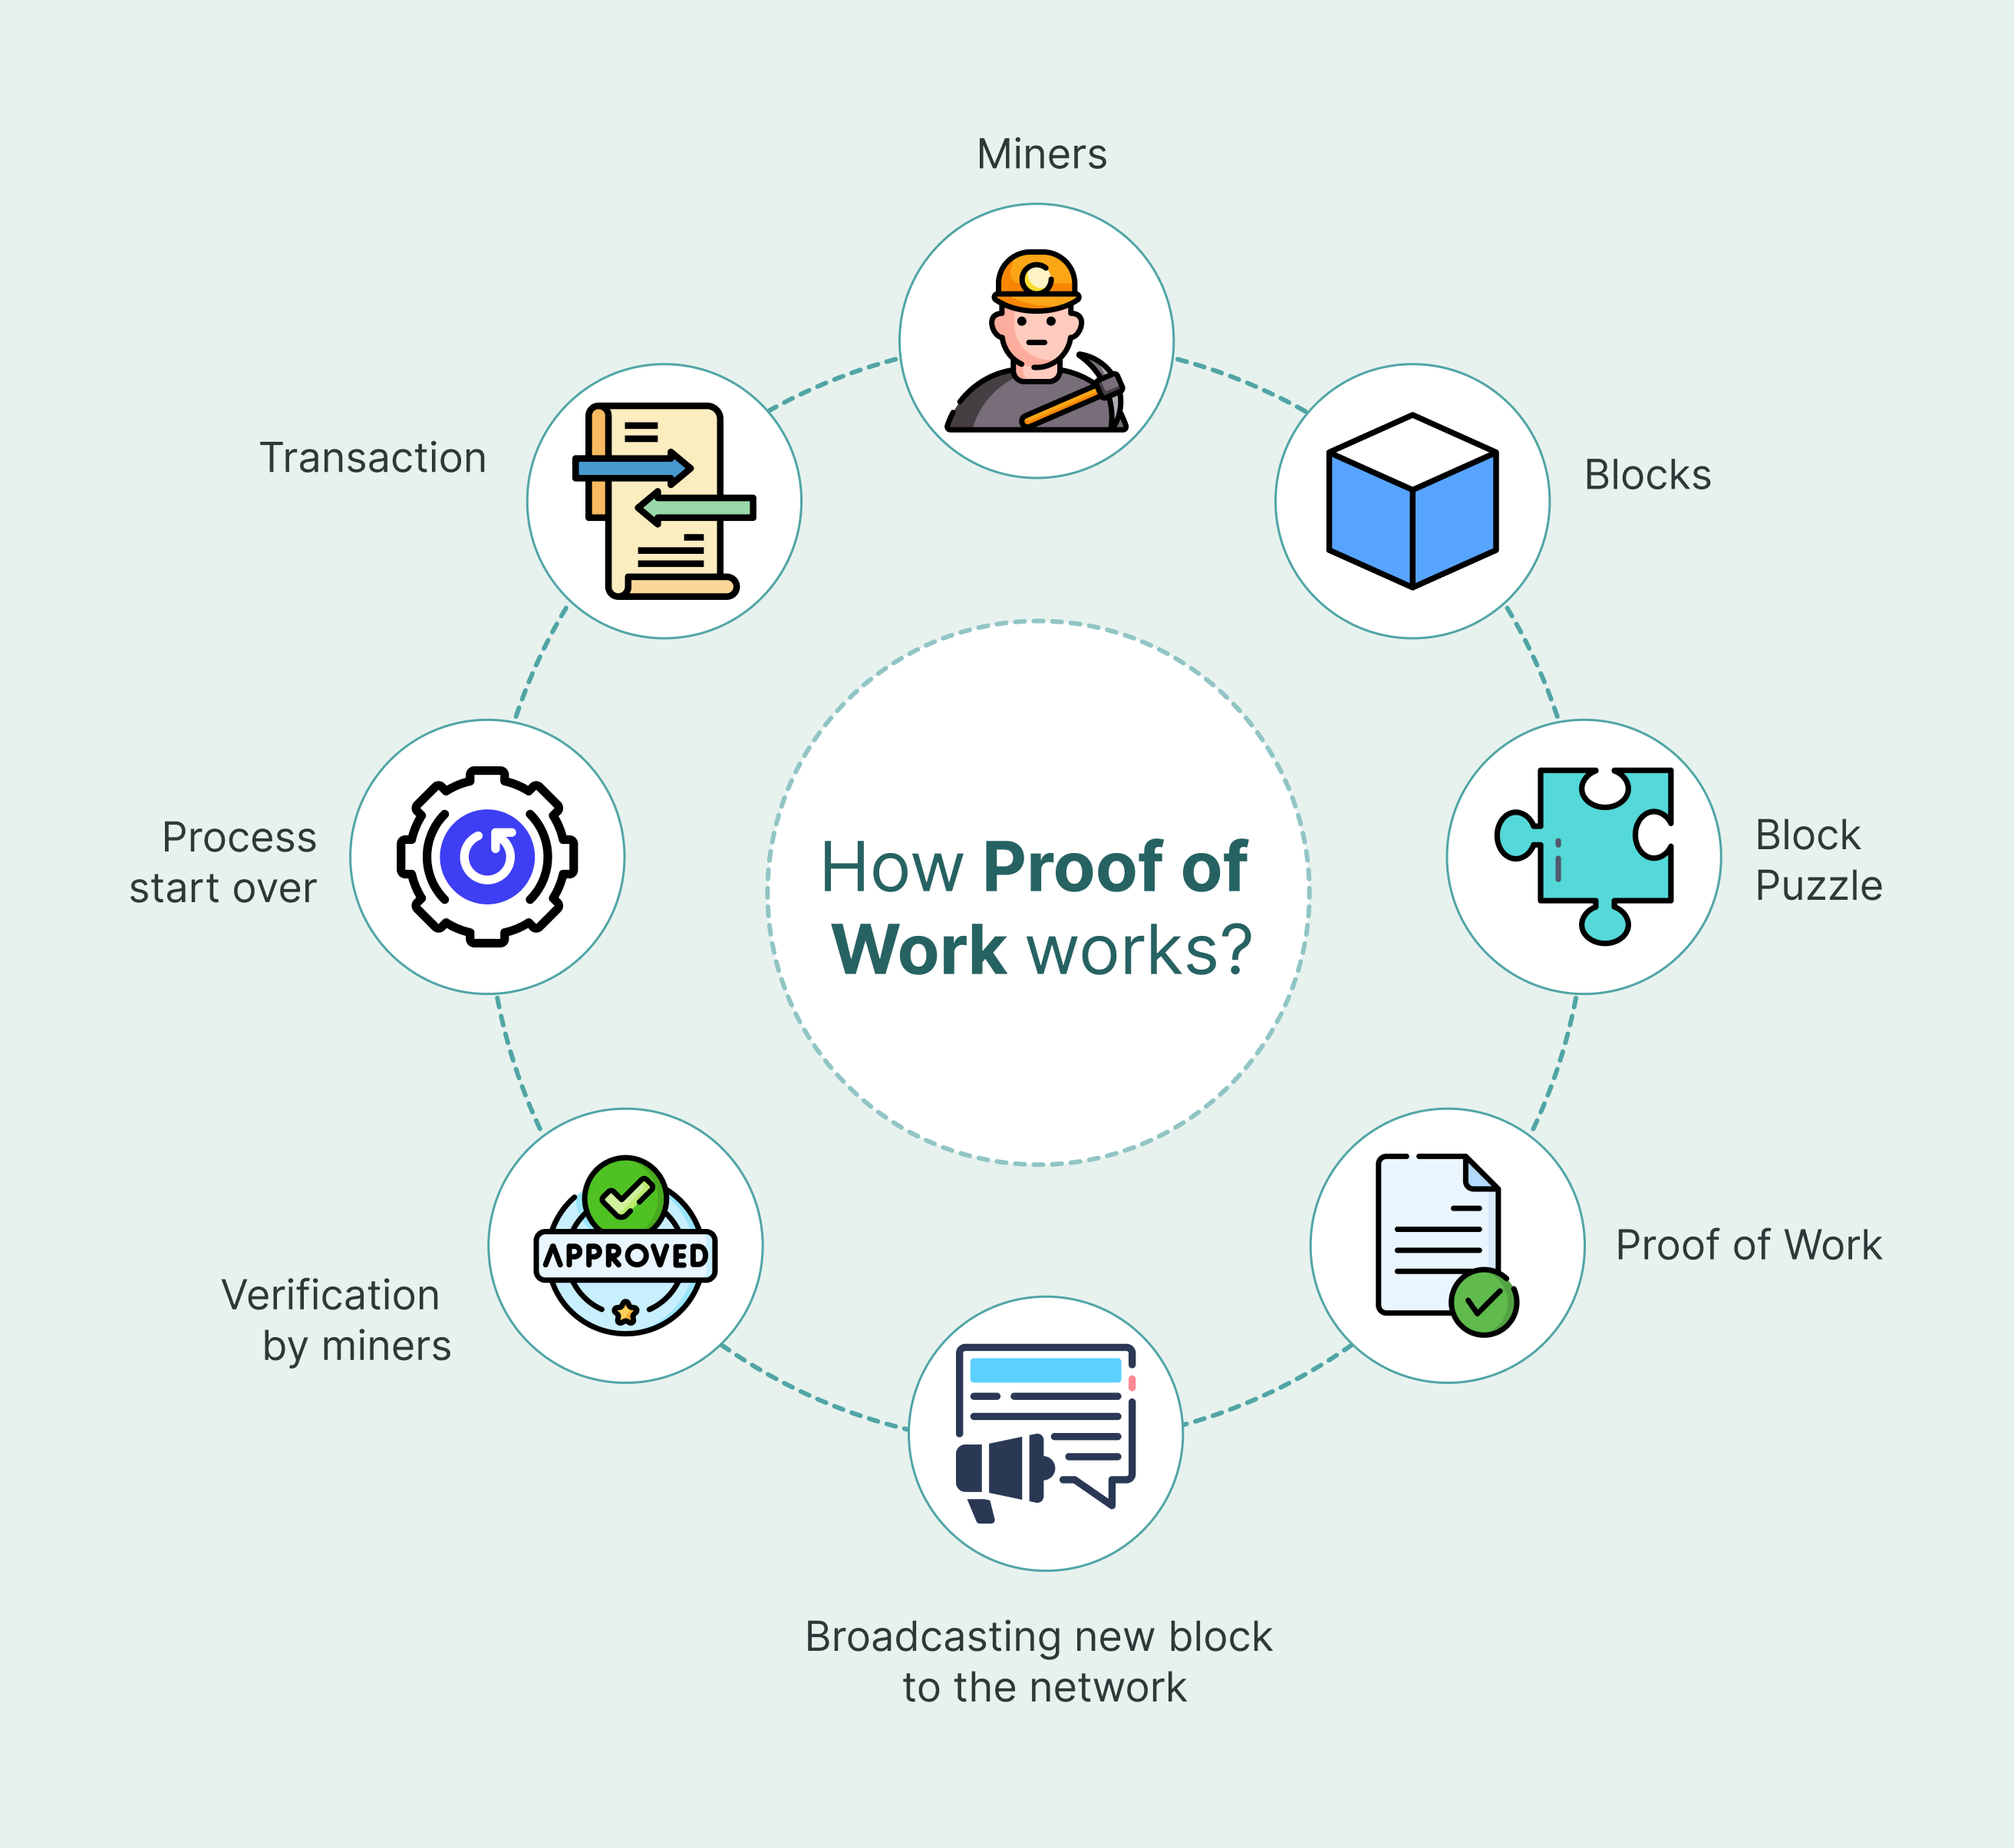
\includegraphics[width=\textwidth]{Images/ConsesnsusProofOfWork.png}
    \caption{Schemat działania Dowodu Pracy}
    \label{fig:ConsesnsusProofOfWork}
\end{figure}
\subsection{Dowód Stawki}
Dowód Stawki (angielski - Proof Of Stake) opiera się na założeniu, że im większą ktoś postawił/położył stawkę na to, że będzie mógł zostać wybrany weryfikatorem tym większe prawdopodobieństwo tego, że zostanie wybrany weryfikatorem. Szczegółowo mówiąc metoda Dowodu Stawki przebiega tak, że po zebraniu odpowiedniej liczby wiadomości tworzony jest blok, lecz aby mógł on zostać utworzony najpierw weryfikatorzy decydują czy wiadomości z bloku są autentyczne i nikt ich nieautoryzowanie nie zmodyfikował. Jeśli większość weryfikatorów postanowi, żeby zbiór wiadomości jest prawidłowy tworzony jest nowy blok. Weryfikatorzy, którzy głosowali uczciwie są nagradzani za swój głos poprzez podarowanie im określonej ilości kryptowaluty (angielski – stacking), a weryfikatorzy, którzy zagłosowali nieuczciwie karani są poprzez zabranie postawionej przez nich stawki (angielski – slashing). Wydawać by się mogło, że ta metoda promuje bogatych użytkowników i umożliwia im oszustwa, lecz w rzeczywistości osoby bogate (te który postawiły najwyższą stawkę) są najbardziej odstraszane od oszustwa, ponieważ w przypadku nieuczciwego zachowania podczas weryfikacji potencjalnego bloku są oni najbardziej karani (ponieważ postawili największą stawkę). Dodatkowo ta metoda konsensus zapewnia duży stopień decentralizacji (w przeciwieństwo do tego do czego w praktyce dochodzi w Dowodzie Pracy). W metodzie tej nie da się oszukać poprzez sytuację, że jedna osoba tworzy wiele kont (sytuacja określana też jako tworzenie multikont), ponieważ w metodzie konsensusu Dowodu Stawki nie chodzi o to ilu użytkowników jest w sieci, a ile postawili oni stawki.

\vspace{0.3\baselineskip}

Działanie Dowodu Stawki na grafice \ref{fig:ConsensusPOS}
\begin{figure}[H]
    \centering
    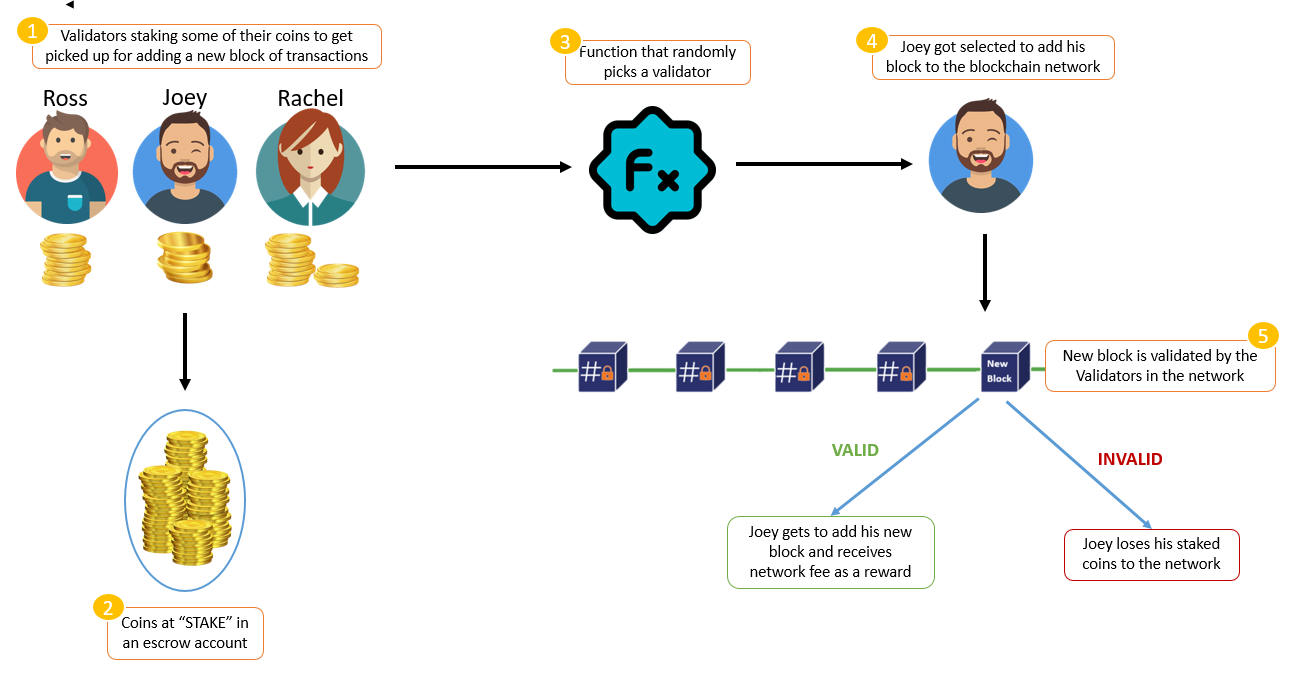
\includegraphics[width=\textwidth]{Images/ConsensusPOS.png}
    \caption{Schemat działania Dowodu Stawki}
    \label{fig:ConsensusPOS}
\end{figure}

\subsection{Delegowany Dowód Stawki}

Delegowany Dowód Stawki (angielski - Delegated Proof Of Stake) działa w podobny sposób jak Dowód Stawki, lecz z tym zastrzeżeniem, że wszyscy użytkownicy sieci zamiast mieć możliwość bycia wylosowanym głosują na jednego z dostępnych delegatów by on podczas weryfikacji głosował w ich imieniu. Nagrody za uczciwe głosowanie dostają delegaci, mogą podzielić się z nimi z użytkownikami, którzy na nich głosowali. Pomimo tego, że ta metoda konsensusu szybsza niż Dowód Stawki jej istotną wadą jest to, że w niej występuje o wiele większa centralizacji i zwykły użytkownik (o ile nie jest delegatem) nie ma bezpośredniej możliwości decydowania o tym czy uważa dany blok za prawidłowy czy też nie).

\vspace{0.3\baselineskip}

Działanie Delegowanego Dowodu Stawki na grafice \ref{fig:ConsensusDPOS}
\begin{figure}[H]
    \centering
    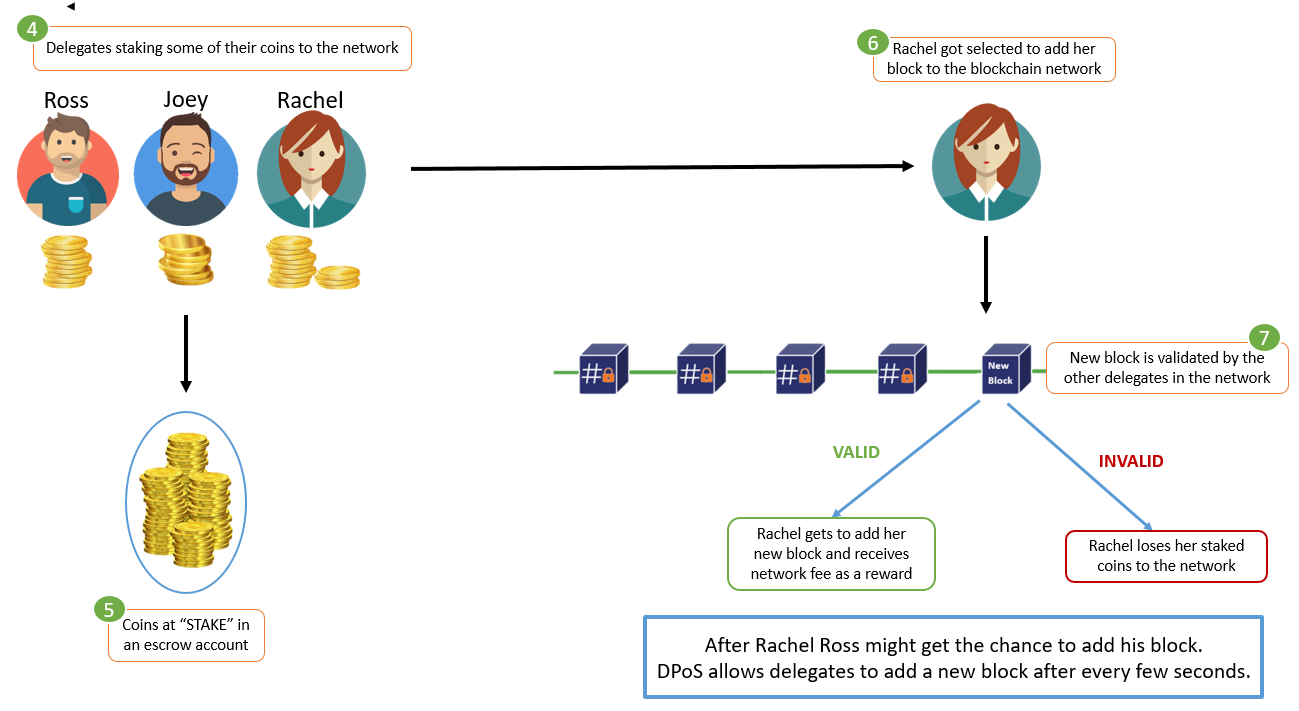
\includegraphics[width=\textwidth]{Images/ConsensusDPOS.png}
    \caption{Schemat działania Delegowanego Dowodu Stawki}
    \label{fig:ConsensusDPOS}
\end{figure}

\subsection{Dowód Pojemności}

W Dowodzie Pojemności (angielski - Proof Of Capacity) każdy z uczestników posiada pliki wykresów, w których są już wcześniej obliczone wartości matematyczne. Podczas tworzenia nowego bloku ogłaszana jest pewna wartość liczbowa i uczestnicy przeszukują swoje pliki wykresów, aby znaleźć wartość najbardziej do niej pasująca. Użytkownik, który będzie miał wartości najbliżej tej poszukiwanej zostanie nagrodzony kryptowalutą. Zaletą tej metody konsensusu jest fakt, że każdy może wziąć w niej udział, ale w rzeczywistości realne szanse mają osoby o ogromnej pojemności pamięciowej, co prowadzi do tworzenia się duży grup/związków tworzonych przez różne organizacje (na przykład firmy) co prowadzi do zwiększenia i dążenie do centralizacji.

\vspace{0.3\baselineskip}

Działanie Dowodu Pojemności na grafice \ref{fig:ConsensusPOC}
\begin{figure}[H]
    \centering
    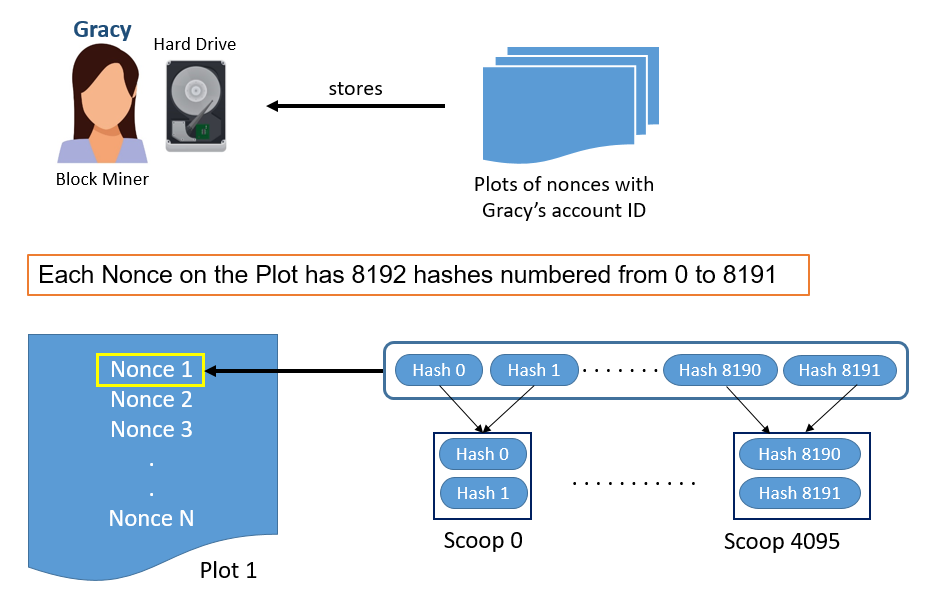
\includegraphics[width=\textwidth]{Images/ConsensusPOC.png}
    \caption{Schemat działania Dowodu Pojemności}
    \label{fig:ConsensusPOC}
\end{figure}

\subsection{Porównanie algorytmów osiągania konsensusu}
Spośród wszystkich dostępnych metod konsensusu wybrano tą która z pozoru wydaje się być nieuczciwie faworyzującą bogatszych uczestników. Dowód Stawki jest jedynym z wyżej wymienionych algorytmów, który nie ma w sobie istotnej wady jaką jest dążenie do centralizacji wywołane stosowaniem konkretnej metody konsensusu – centralizacji jednostek obliczeniowych (Dowód Pracy), centralizacji pojemności pamięciowej (Dowód Pojemności) czy centralizacji możliwość decydowania o poprawności danego bloku jedynie dla wybranej grupy osób (Delegowany Dowód Stawki). Dowód Stawki w przeciwieństwie do niektórych z innych algorytmów osiągania  konsensusu nie powoduje nadmiernego zużywania zasobów – prądu używanego do obliczeń w Dowodzie Pracy i przestrzeni dyskowej (w tym sprzętu elektronicznego) by zwiększyć ilość posiadanej pamięci w Dowodzie Pojemności. Wracając do zarzutu stawianego Dowodowi Stawki na początku akapitu co prawda najbogatsi (posiadający największą stawkę) mają największe szanse na zostanie weryfikatorem, ale w przypadku oszustwa są oni najmocniej karani, ponieważ tracą całą swoją postawioną stawkę (zjawisko to nazywa się slashing).

\subsection{Użycie algorytmów osiągania konsenusu w praktyce}
\begin{lstlisting}[caption={Wybieranie osoby mającej zostać weryfikatorem}]
def drawVerifier(self):
    personStakeList = []
    for peer in self.peers:
        personValue = {"addr": peer.addr, "port": peer.port,
        "stake": peer.stake}
        personStakeList.append(personValue)
    myValue = {"addr": ip(), "port": self.port, "stake": self.stake}
    personStakeList.append(myValue)
    personStakeList.sort(key=lambda x: x["port"])
    personSingleList = [{k: v for k, v in d.items() if k != "stake"} 
    for d in personStakeList]
    stakeSingleList = [x["stake"] for x in personStakeList]
    keyRaw = " ".join(str(x["port"]) for x in personStakeList)
    self.drawString = keyRaw
    numeric_seed = int.from_bytes(hashlib
    .sha256(keyRaw.encode('utf-8')).digest())
    random.seed(numeric_seed) #zmiana seeda dla losowania weryfikatora
    chosen_port = random.choices(personSingleList, 
    weights=stakeSingleList, k=1)[0]
    return chosen_port
\end{lstlisting}
\listings{Wybieranie osoby mającej zostać weryfikatorem}
Przy wybieraniu osoby, która będzie weryfikatorem korzysta się z funkcji, która ma go wyłonić kierując się zasadami z Dowodem Stawki. Problemem jaki nasuwa się przy implementowaniu funkcji jest to, jak sprawić, że każdy będzie miał wylosowanego tego samego weryfikatora, mimo tego, że uruchomienia programu są niezależne od siebie. Wywołanie u każdego z użytkowników zwykłej funkcji losującej wydaje się być nasuwającym się rozwiązaniem, lecz w rzeczywistości może doprowadzić to do sytuacji, gdzie różne osoby będę uznawały różnych członków sieci za weryfikatorów, co jest sytuacją, której chcemy uniknąć. Aby rozwiązać ten problem trzeba posłużyć się niezmiennikiem jakim jest założenie, że przy dowolnej komunikacji grupowej każdy z członków jest połączony z innymi użytkownikami w grupie (na tym polega rozmowa grupowa), ta sytuacja może być chwilowo zaburzona, ponieważ, łączenie się nie zawsze występuje w tym samym czasie, ale system domyślnie dąży do tego stanu.

\begin{lstlisting}[caption={Zamiana łańcucha znaków na wartość liczbową}]
numericSeed = int.from_bytes(hashlib.sha256(keyRaw
.encode('utf-8')).digest())
random.seed(numeric_seed)
\end{lstlisting}
\listings{Zamiana łańcucha znaków na wartość liczbową}

Dalej w kodzie z pozoru mało istotna funkcja skrótu, która zamienia łańcuch znaków na wartość liczbową. W rzeczywistości jest bardzo ważna, ponieważ jeśli jest ona niedeterministyczna (dla tego samego łańcucha znaków wylosuje ona różną wartość liczbową) to wyłanianie weryfikatora będzie mijać się z celem, bo wtedy nie wszyscy będą mieli tego samego weryfikatora. Skoro zostało wspomniane, dlaczego deterministyczna funkcja skrótu jest tak ważna, to warto wspomnieć, że domyślna funkcja skrótu w Pythonie – hash() – nie jest funkcją deterministyczną, ponieważ wprowadzono do niej mechanizm losowości skrótu (angielski - hash randomization) który dodaje do funkcji skrótu losową ,,sól”. Z tego powodu w systemie zastosowano metodę hashlib.sha256(), która jest deterministyczna. Następnie tak utworzoną liczbą ustawiamy ziarno generatora liczb pseudolosowych tak, aby generator dla tych samych danych wejściowych dał nam takie same wyniki.

\begin{lstlisting}[caption={Losowanie weryfikatora}]
chosen_port = random.choices(personSingleList, 
weights=stakeSingleList, k=1)[0]
return chosen_port
\end{lstlisting}
\listings{Losowanie weryfikatora}

Następnie odbywa się losowanie weryfikatora, jako zgodne z metodą uzyskania konsensusu Dowodu Stawki jest wylosowanie jednego z uczestników, ale nie za pomocą zwykłej metody random.choice w Pythonie, która losowałaby elementy z listy z równym prawdopodobieństwem, ale z metodą random.choices, której argumentem (poza listą członków sieci), jest lista wartości postawionych przez nich jako stawki i jest ona stosowana jako lista wag, to znaczy im ktoś większą postawił stawkę, tym większa jest jego szansa na zostanie wylosowanym, co jest zgodne z założeniami Dowodu Stawki.

\section{Metody zabezpieczania bloku}

Gdy zestaw wiadomości został zweryfikowany jako prawidłowy i tworzony jest z nich blok, pojawia się wątpliwość jak zabezpieczyć blok przed nieautoryzowanymi zachowaniami  (zmianami treści wiadomości), tak aby każdy członek sieci mógł w łatwy sposób sprawdzić czy faktycznie, nikt nie zmodyfikował wiadomości (na przykład w celu oszustwa, które ma mu przynieść korzyść).

\subsection{Zabezpieczanie bloku w Dowodzie Pracy}

W metodzie konsensusu Dowód Pracy poprawność bloku sprawdza się poprzez porównywanie funkcji skrótu odpowiednio ze sobą połączonych bloków. Wadą tego rodzaju rozwiązania jest fakt, że do samego sprawdzenia podpisu potrzebne są ogromne moce obliczeniowe, co jest mocno nie korzystne i dodatkowo jednostka lub zespół jednostek posiadający odpowiednio dużą moc obliczeniową może zamienić treści wiadomości w poprzednich blokach w łańcuchu tak, aby wartość funkcji skrótu się zgadzała z nowszymi wiadomościami i nie wzbudzała podejrzeń.

\vspace{0.3\baselineskip}

Łączenie bloków w Dowodzie Pracy za pomocą funkcji skrótów na grafice \ref{fig:ProofOfWorkHash}
\begin{figure}[H]
    \centering
    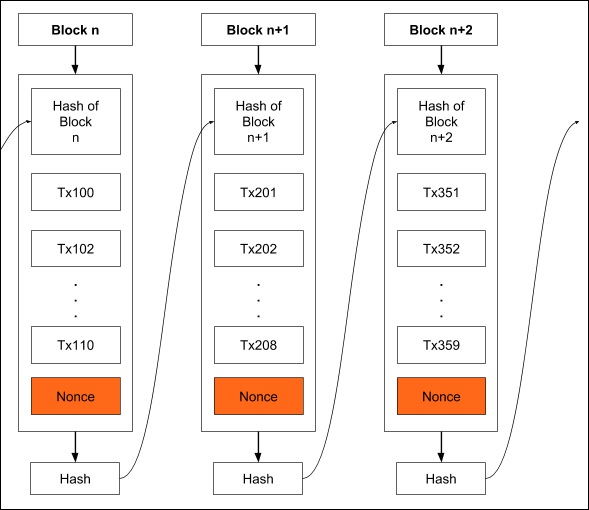
\includegraphics[width=\textwidth]{Images/ProofOfWorkHash.jpg}
    \caption{Działanie funkcji skrótu w Dowodzie Pracy}
    \label{fig:ProofOfWorkHash}
\end{figure}

Zamiast stosować skomplikowany połączonych ze sobą funkcji skrótu w implementacji systemu postanowiono skorzystać z innej metody, również stosowanej w innych systemach kryptograficznych. Jest to podpis cyfrowy.

\subsection{Zabezpieczanie bloku poprzez podpis cyfrowy}

Podpis cyfrowy opiera się na kryptografii asymetrycznej, gdzie każdy z użytkowników ma dwa klucze – klucz publiczny i klucz prywatny. W podpisie cyfrowym najpierw wykonuje się funkcję skrótu (w implementacji stosuje się SHA-256) na danych znajdujących się w bloku. Potem tą wartość szyfruje się kluczem prywatnym. Podpis cyfrowy (w przeciwieństwie do szyfrowania) jest wykonywany kluczem prywatnym, ponieważ jeśli weryfikator po otrzymaniu wartości funkcji skrótu próbował podpisać ją kluczem publicznym to żaden z użytkowników nie miałby możliwości zweryfikowania takiego podpisu, ponieważ do to tego potrzebny jest drugi klucz, czyli klucz prywatny, ale założeniem kryptografii asymetrycznej jest to, że klucz prywatny jest niedostępny dla innych. 

Zilustrowanie podpisu cyfrowego na grafice \ref{fig:DSJP}:
\begin{figure}[H]
    \centering
    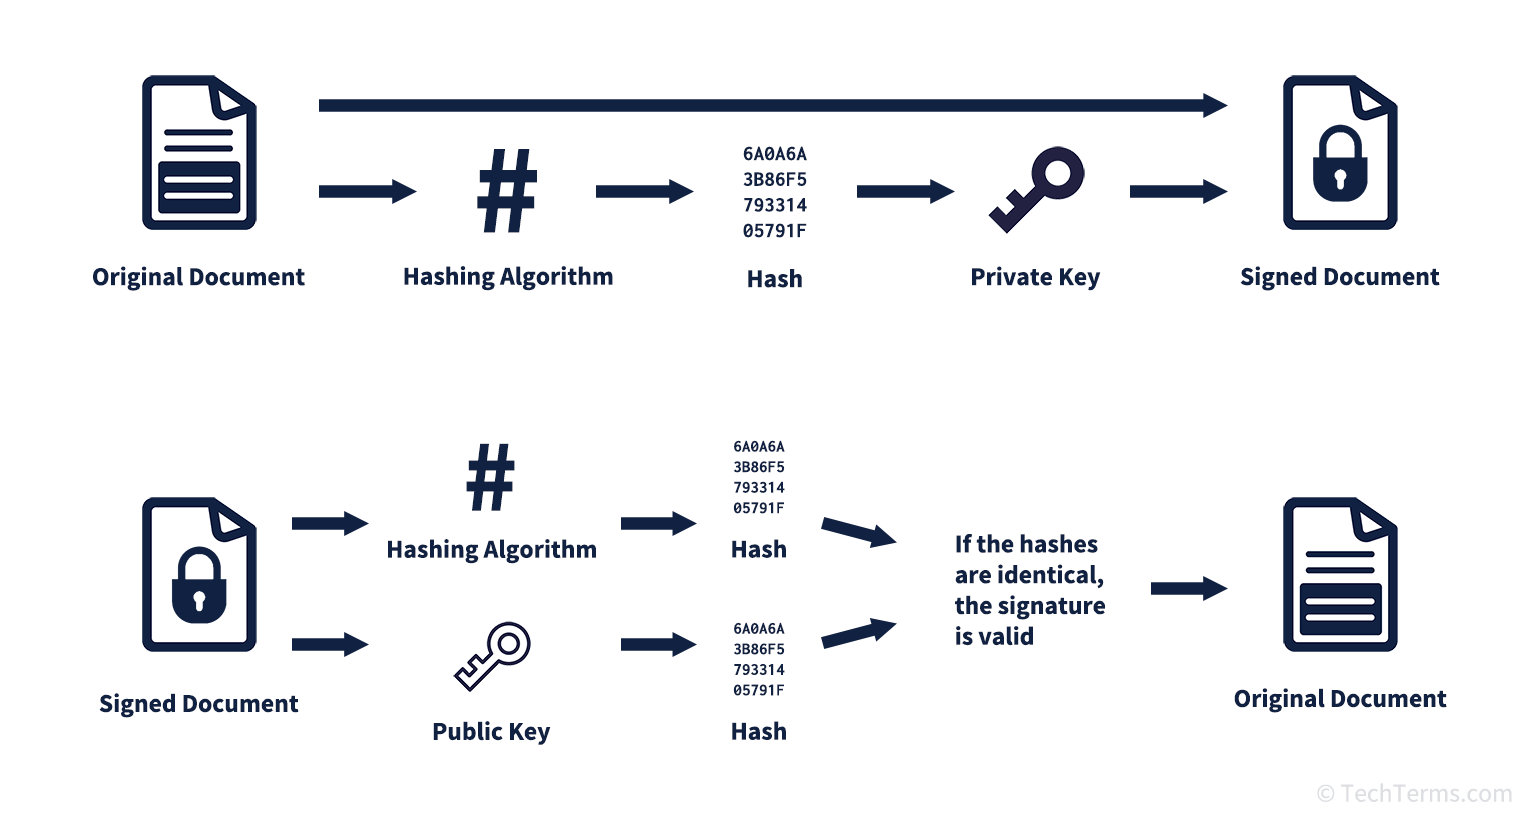
\includegraphics[width=\textwidth]{Images/DSJPG.jpg}
    \caption{Działanie podpisu cyfrowego}
    \label{fig:DSJP}
\end{figure}

Aby zweryfikować podpis cyfrowy należy wygenerować hash z danych znajdujących się w bloku. Jeśli ta wartość jest tożsama z wartością podpisu cyfrowego odszyfrowanego kluczem publicznym twórcy podpisu to znaczy, że podpis jest autentyczny.

\subsection{Zabezpieczanie bloku w praktyce}

\begin{lstlisting}[caption={Wysyłanie podpisu elektronicznego}]
def sendDigitalSignature(self, ListOfJSON, me):
    jsonMessages = self.get_messages_block(ip())
    drawnVerifier = self.drawVerifier()
    if drawnVerifier == self.port:
        me.remove_single_message_JSON(ip())
        for count, jsonSingleMessage in enumerate(jsonMessages):
            if jsonMessages[count] == ListOfJSON[0]:
                length = len(ListOfJSON)
                identicalResult = jsonMessages[count:count+length]
                                == ListOfJSON
                if identicalResult:
\end{lstlisting}
\listings{Wysyłanie podpisu elektronicznego}
Jeżeli dany użytkownik został wylosowany jako weryfikator, a następnie jeśli otrzymane wiadomości (od osoby wysyłającej ostatnią wiadomość w bloku) zgadzają się z wiadomościami, które posiada weryfikator to potwierdza je on za pomocą wystawienia podpisu cyfrowego.

\begin{lstlisting}[caption={Tworzenie podpisu elektronicznego}]
def createSignature(self, dataStrng):
    data = dataStrng.encode('utf-8')
    signature = self.private_key.sign(
        data,
        padding.PKCS1v15(),
        hashes.SHA256()
    )
    return signature
\end{lstlisting}
\listings{Tworzenie podpisu elektronicznego}
Następnie tworzony jest podpis cyfrowy na podstawie przekazanych wiadomości w formie łańcucha znaków. Szczegółowo, że łańcuch znaków przekształcany jest do postaci binarnej, potem te dane binarne są podpisywane przy wykorzystaniu klucza prywatnego. Poza samymi danymi innymi argumentami w schemacie podpisu cyfrowego jest wypełnienie (angielski – padding) – tu używane jest schemat PKCS1v15. Innym argumentem do funkcji podpisu cyfrowego jest określona funkcja skrótu, ponieważ podpisywanie całego ciągu znaków binarnych byłoby zbyt czasochłonne, w tym przypadku zastosowano algorytm SHA256. Podczas implementacji może pojawić się wątpliwość czy każdy z użytkowników będzie mógł dla tych samych danych otrzymać taki sam podpis cyfrowy i czy przy weryfikacji podpisu cyfrowego dla tych samych danych otrzyma ten sam wynik. Jest to kluczowe dla działania programu, jeśli to nie zostałoby to zapewnione weryfikacji podpisu cyfrowego byłaby nie możliwa. Pożądana przez nas cecha algorytmu, czyli fakt, że dla tych samych danych algorytm zawsze zwróci ten sam wynik to deterministyczność. Jak sprawdzić czy nasz podpis cyfrowy jest deterministyczny – trzeba dowiedzieć się czy funkcja go tworząca zwraca deterministyczny wynik, a faktem jest informacja, że w tej funkcji jest to uzależnione od tego jakie wypełnienie jest stosowane oraz jaki algorytm generowania funkcji skrótu jest stosowany. Co do metody wypełnienia PKCS1v15 – jest ona deterministyczna (nie stosuje ona elementów losowanych w przeciwieństwie do wielu innych metod wypełnienia), funkcja skrótu SHA256 (w przeciwieństwie do niektórych innych funkcji skrótu) jest deterministyczna. Ukazując, to że metoda wypełnienia jak i funkcja skrótu są deterministyczne, ukazane jest, że funkcja generująca podpis cyfrowy, która od nich bezpośrednio zależy również jest deterministyczna, więc udowodniono, że podpis cyfrowy jest deterministyczny (taki sam dla identycznych danych wejściowych).

\section{Algorytmy kodowania transportowego}
\subsection{Opis algorytmów kodowania transportowego}
Podczas przesyłania danych przez sieć może pojawić się problem, że niektóre dane (na przykład podpis cyfrowy czy klucz publiczny) są w postaci ciągu bajtów. Ich przesyłanie przez sieć w formie binarnej jest dość problematyczne, więc dobrym rozwiązaniem problemu jest ich przekonwertowanie na format danych, który można w łatwiejszy sposób przesłać jak na przykład łańcuch znaków. Można wykonywać to ręcznie, ale lepszym rozwiązaniem jest skorzystanie z gotowego algorytmu kodowania transportowego. Istnieje wiele algorytmów kodowania transportowego, takie jak Base16, Base32, Base36, Base62 czy Base64 czy Base85. W implementacji projektu został wybrany jeden z najbardziej znanych i efektywnych algorytmów kodowania transportowego, czyli Base64. Jego działanie polega na tym, że dzieli on ciąg bajtów na trzy-bajtowe grupy, które są potem dzielone na cztery sześciobitowe grupy, a każda z tych sześciobitowych grup jest zamieniana na jedną liczbę. Liczba ta jest uzyskiwana mnożąc bity od najmłodszego do najstarszego przez kolejną potęgę liczby dwa według wzoru \ref{eq:Base64Formula}
\begin{equation}
    Liczba = \sum_{i=1}^6 bit_i * 2^{i-1}
    \label{eq:Base64Formula}
\end{equation}
\equations{Liczba w kodowaniu Base64}
Podział ciągu bajtów na trzybajtowe grupy, na następnie na cztery sześciobitowe grupy został zwizualizowany, na grafice \ref{fig:Base64Schema}
\begin{figure}[H]
    \centering
    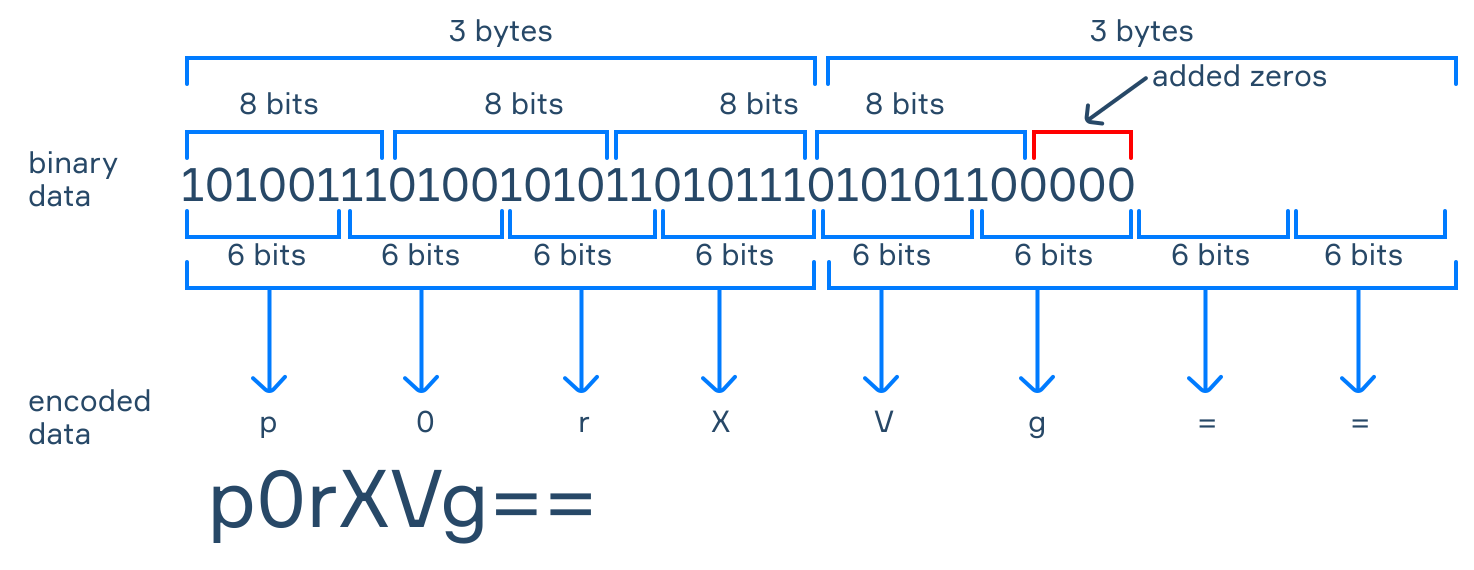
\includegraphics[width=\textwidth]{Images/Base64Schema.png}
    \caption{Schemat Base64}
	\label{fig:Base64Schema}
\end{figure}
Potem liczba ta konwertowana jest na jeden z sześćdziesięciu czterech znaków ASCII (jest to cyfra od 0 do 9, albo wielka litera od A do Z, albo mała litera od a do z, albo znak plusa lub równości). Odbywa się to zgodnie ze schematem pokazanym na grafice \ref{fig:Base64Coding}
\begin{figure}[H]
    \centering
    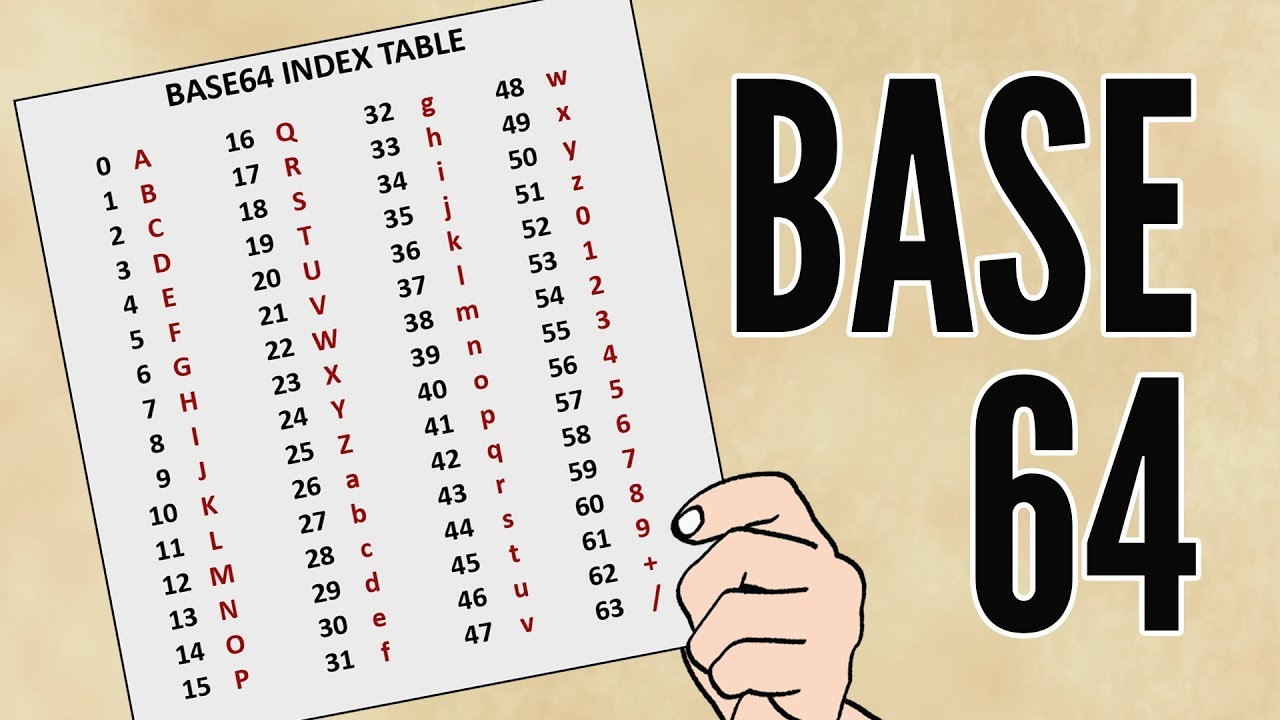
\includegraphics[width=\textwidth]{Images/Base64Coding.jpg}
    \caption{Kodowanie w Base64}
	\label{fig:Base64Coding}
\end{figure}
Na ciągu znaków w formacie Base64 można również wykonać operację odwrotną, czyli zdekodować go do postaci binarnej.

\vspace{0.3\baselineskip}

Jeśli długość ciągu bajtów nie jest liczbą podzielną przez trzy stosuje się dopełnienie, która zamiast wcześniej opisanych sześdziesięciu czterech znaków dodaje znaki równości tak, żeby liczba znaków po konwersji była liczbą podzielną przez cztery.